    % ===========================================================================
    % Section 4: Experiments
    % ===========================================================================
    
    \begin{figure*}[htbp!]
      \centering
      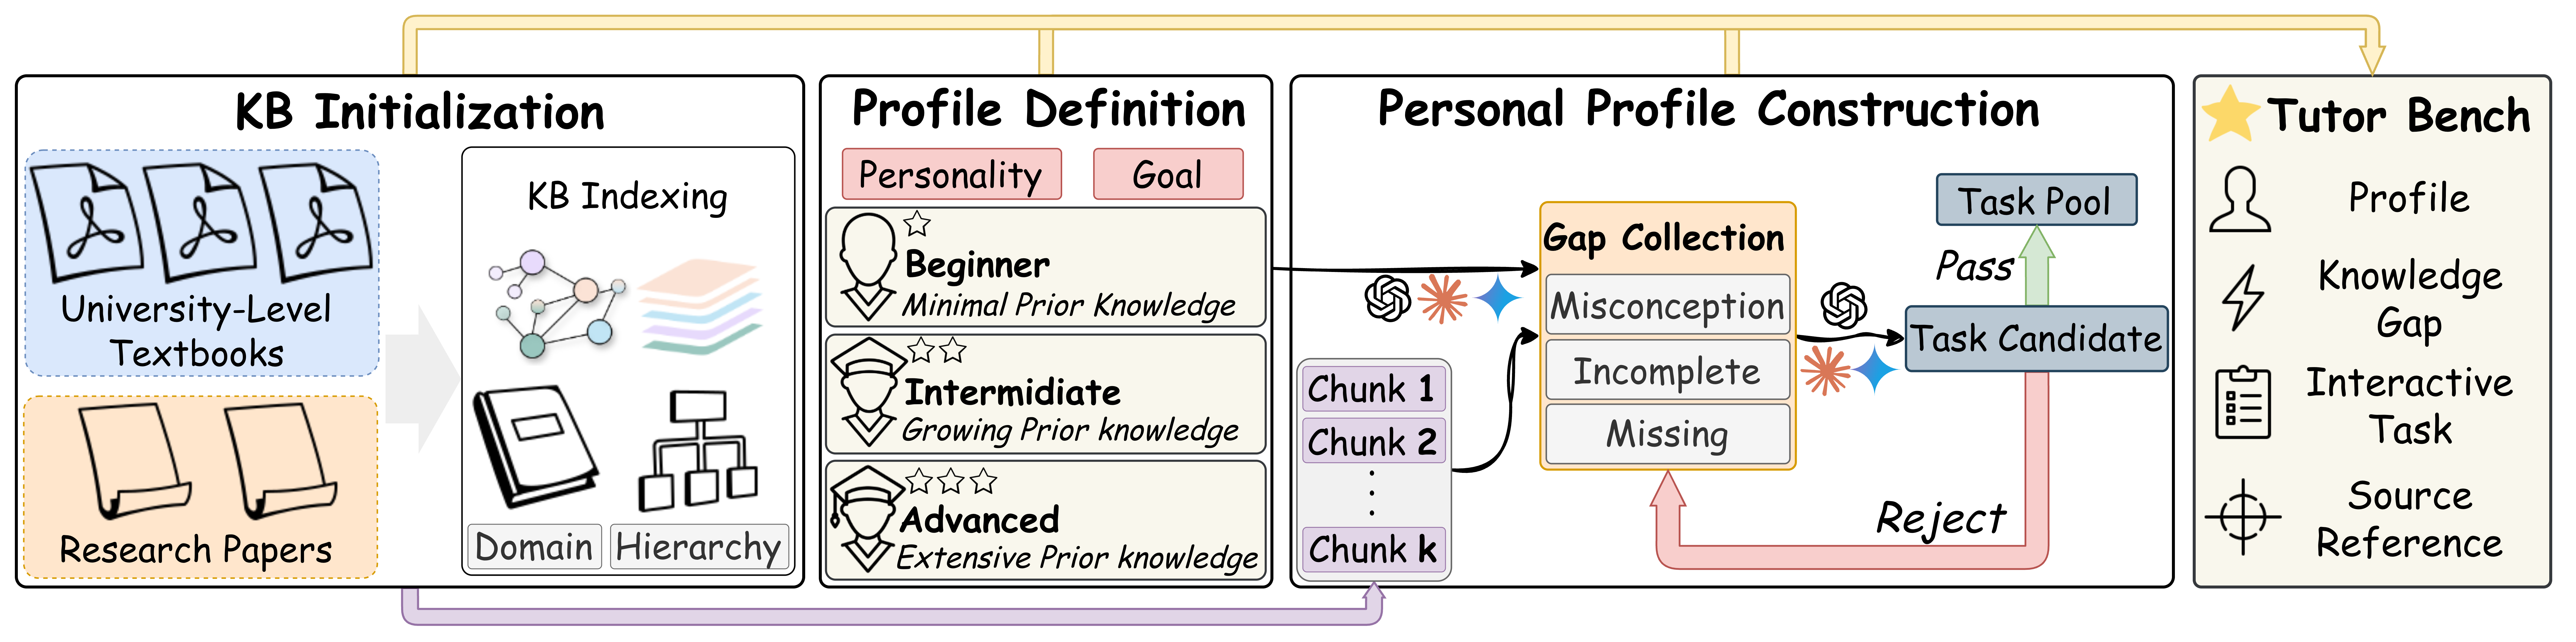
\includegraphics[width=\textwidth]{figures/data-gen-ver2.png}
      \caption{Construction pipeline of \textbf{TutorBench}. Four stages---KB Initialization, Profile Definition, Personal Profile Construction (with grounded knowledge gaps and rejection sampling), and final assembly---produce entries each containing a learner profile, knowledge gaps, an interactive task, and source references.}
      \label{fig:datagen}
  \end{figure*}
  
  
  \section{Experiments}
  \label{sec:experiments}
  
Conventional QA-style benchmarks mostly measure final correctness, but personalized tutoring requires process-level evaluation: whether the system diagnoses learner-specific gaps, corrects them through interaction, and then generates targeted follow-up practice.
Accordingly, we evaluate \textsc{DeepTutor} along three axes:
\textbf{TutorBench} construction quality (\S\ref{sec:tutorbench}),
\textbf{first-person interactive tutoring quality} (\S\ref{sec:interactive_eval}),
and \textbf{general problem-solving transfer} (\S\ref{sec:generalization}).
  
  
  % ===========================================================================
  \subsection{TutorBench: A Personalized Tutoring Benchmark}
  \label{sec:tutorbench}
  % ===========================================================================
  
Existing educational benchmarks rarely model who the student is and what they specifically misunderstand.
We construct \textbf{TutorBench}, where each entry explicitly couples a learner persona, grounded knowledge gaps, and an interactive tutoring task.
The construction pipeline is shown in Figure~\ref{fig:datagen}.
  
  \paragraph{KB Initialization.}
  University-level textbooks and research papers are indexed into the dual-representation knowledge base described in \S\ref{sec:rag}.
  A \textit{domain hierarchy} is simultaneously derived from the document structure, providing topical scaffolding for subsequent profile generation.
  
\paragraph{Profile Definition.}
Each KB instantiates three learner profiles---\textit{beginner}, \textit{intermediate}, and \textit{advanced}---with distinct educational background, learning purpose, and per-topic mastery states (\textit{known well}/\textit{partially known}/\textit{unknown}).
This mirrors the benchmark generator configuration used in the codebase.
  
\paragraph{Personal Profile Construction.}
For each profile, we sample source pages from the KB and generate three types of \emph{grounded knowledge gaps}:
  \textbf{misconceptions} (incorrect beliefs),
  \textbf{incomplete understanding} (partial grasp with missed edge cases), and
  \textbf{missing knowledge} (never-encountered concepts).
  Each gap is anchored to specific source pages and includes both a \textit{manifestation} (how the student would exhibit the gap) and the \textit{correct understanding} for evaluation reference.
  
Gaps are assembled into \textbf{interactive tasks} via rejection sampling that verifies task--gap consistency, source grounding, and conversational naturalness.
  
\paragraph{Statistics.}
TutorBench is generated with a fixed, configuration-driven recipe.
For each KB, we instantiate three learner profiles (\textit{beginner},
\textit{intermediate}, \textit{advanced}), yielding $3 \times N_{\text{KB}}$
profiles in total. We sample source pages to generate at least 3 knowledge gaps for each interactive task and construct 3
interactive tasks per profile via rejection sampling. In our current release, this produces 90 KB-grounded learner
profiles overall, which is 270 interactive tasks.
  
  
  % ===========================================================================
  \subsection{First-Person Interactive Evaluation}
  \label{sec:interactive_eval}
  % ===========================================================================
  
Static evaluation cannot capture whether a tutor adaptively resolves misconceptions over turns.
We therefore use a \textbf{first-person interactive protocol}: an LLM student simulator (initialized from TutorBench entries) interacts with each evaluated system, and we score both dialogue behavior and generated practice questions (Figure~\ref{fig:evaluation}).
  
  \begin{figure}[t]
      \centering
      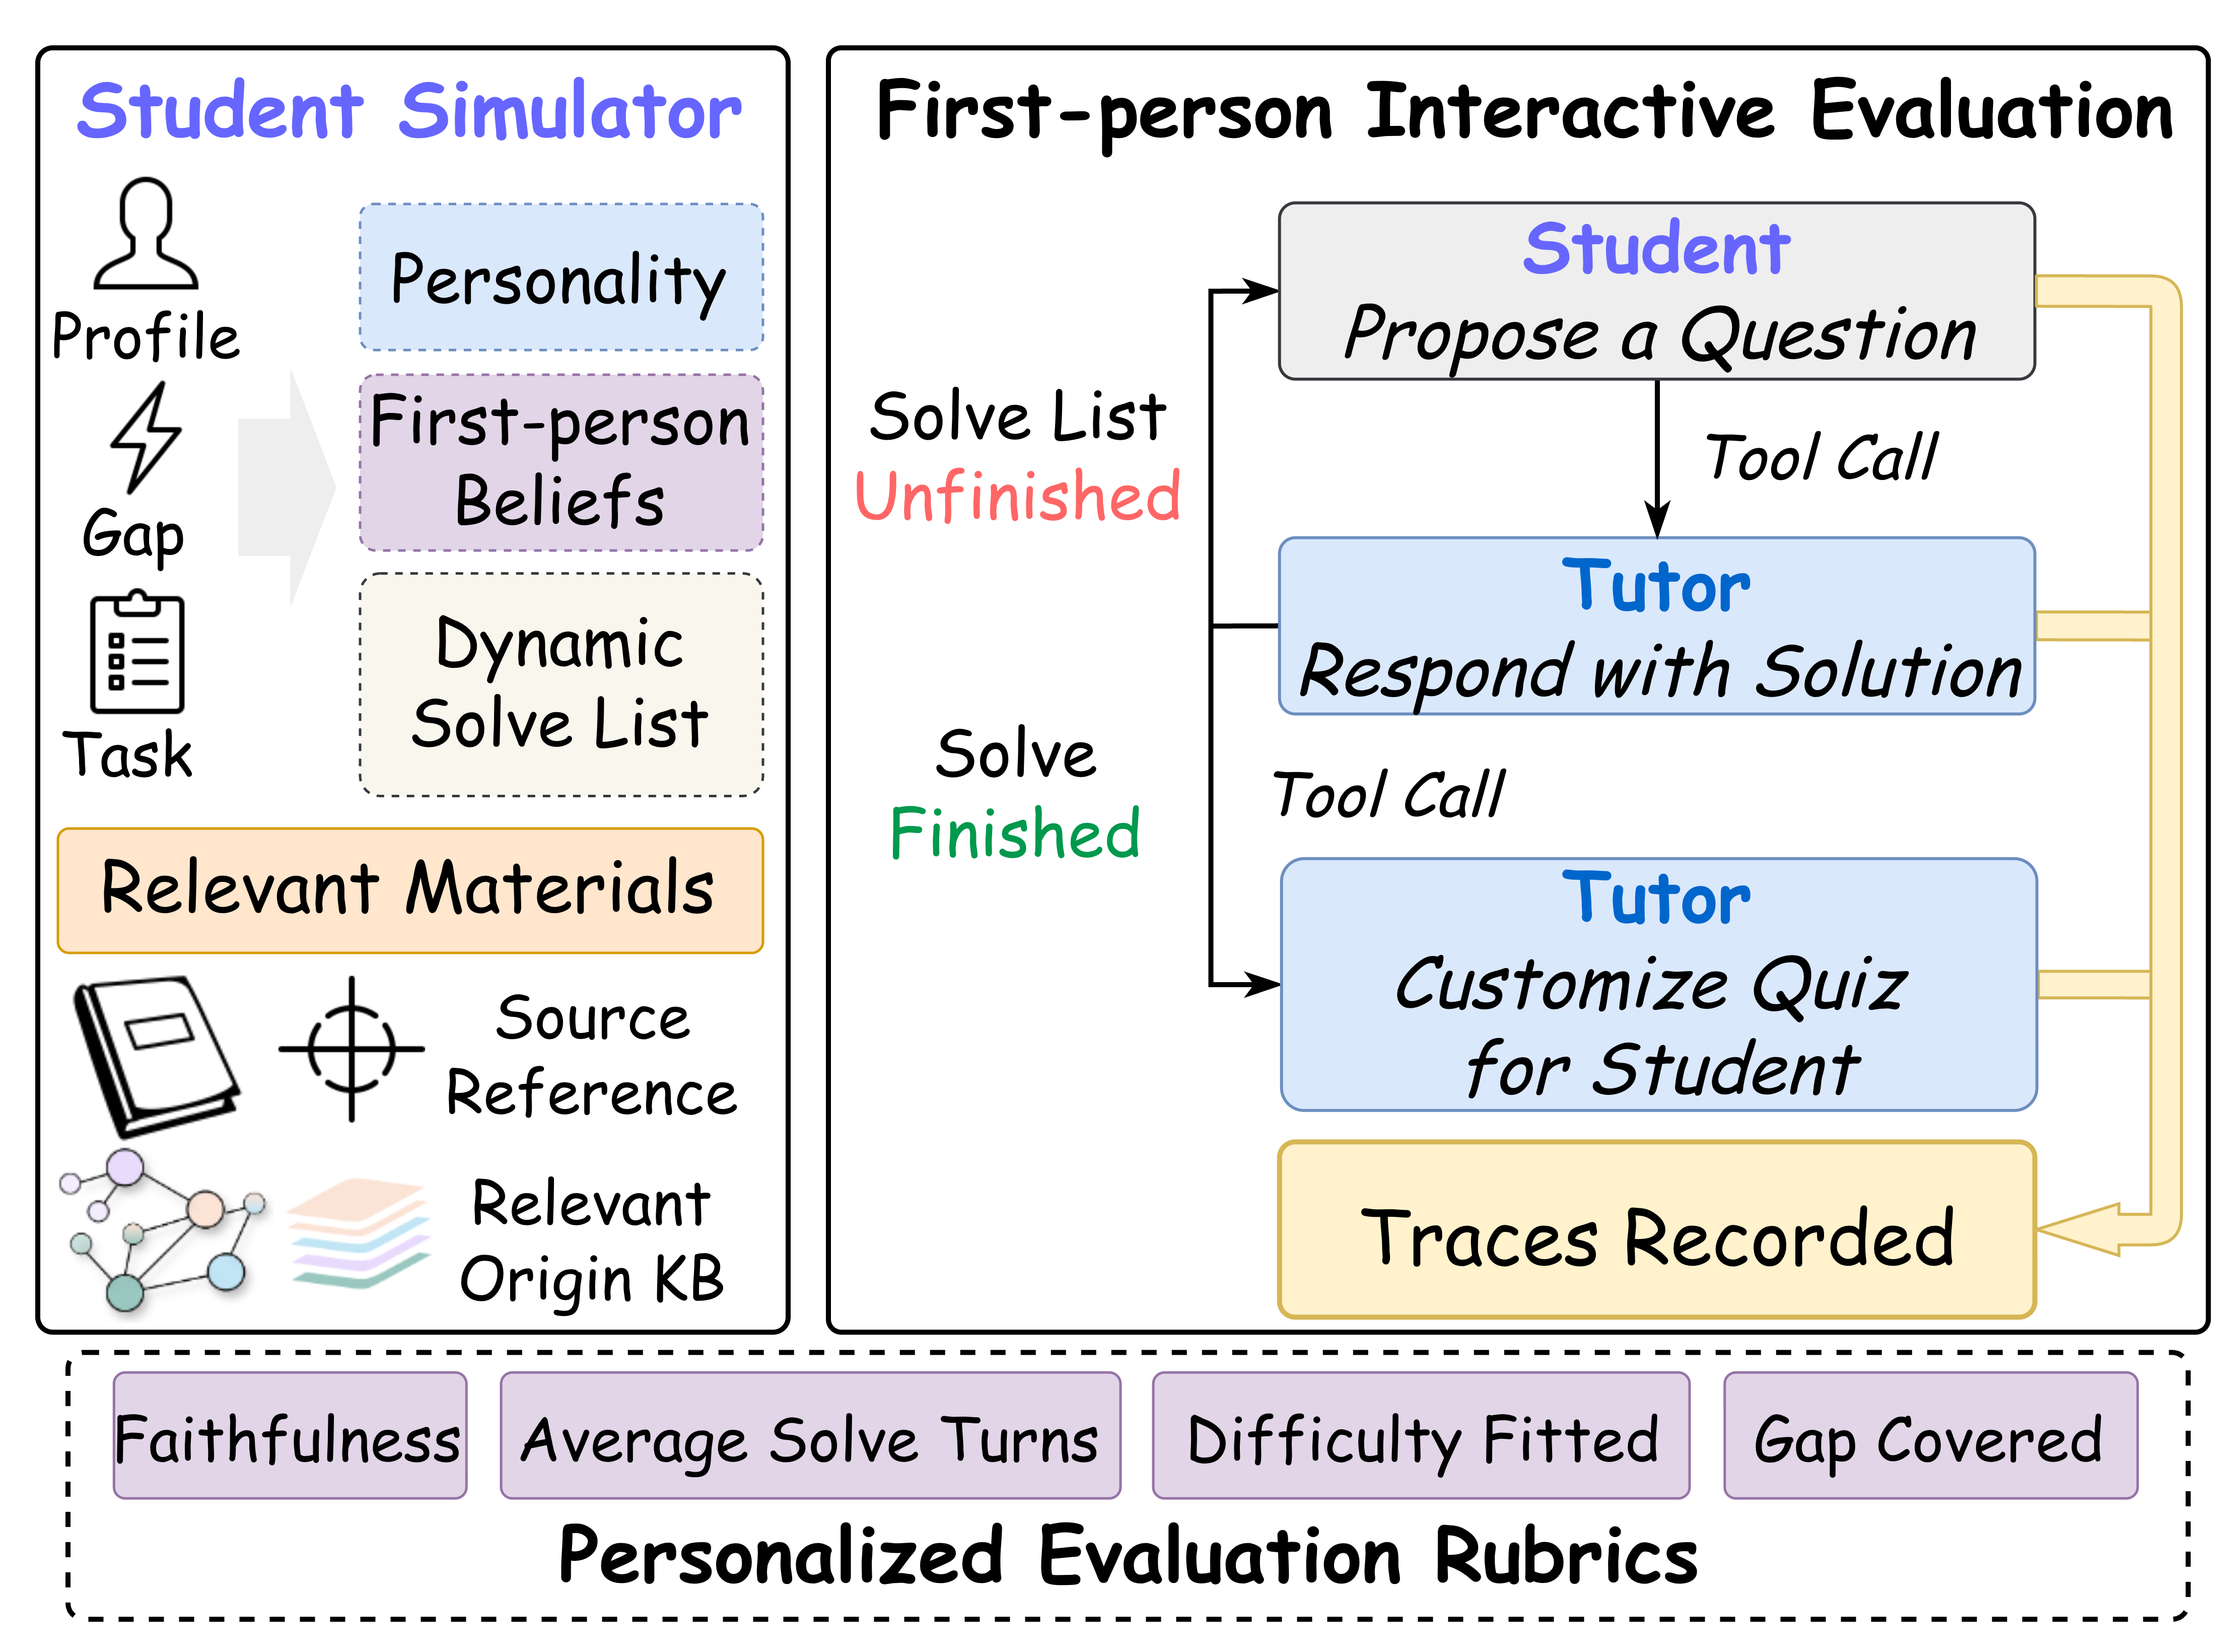
\includegraphics[width=\columnwidth]{figures/evaluation-ver1.png}
    \caption{First-person interactive evaluation protocol. A \textbf{Student Simulator} initialized from TutorBench (persona + first-person gap beliefs + dynamic gap pacing) interacts with the tutor. After session completion, the tutor generates five practice questions. Evaluation is split into \textbf{turn-level tutoring metrics} and \textbf{practice-question metrics}, then aggregated in a fixed-judge Step-3 pipeline.}
      \label{fig:evaluation}
  \end{figure}
  
\paragraph{Student Simulator.}
Each gap is transformed into a first-person belief so the simulator \emph{acts as the student} rather than describing errors from an outside view.
Combined with dynamic gap pacing, this yields realistic resistance patterns: the student may defend misconceptions, partially accept corrections, and only mark completion after sufficient explanation.
  
\paragraph{Evaluation Rubrics.}
Following the latest evaluation pipeline, metrics are explicitly split into
\textbf{turn-level tutoring metrics} and \textbf{practice-question metrics}.
Importantly, the final practice-question turn is \emph{excluded} from turn-level scoring and evaluated independently.
  
  \begin{itemize}[nosep,leftmargin=*]
\item \textbf{Iter}: raw turn count from interactive sessions (lower is better). This is the only non-1--5 metric.
  
\item \textbf{Solve-side Quality}: per-turn 1--5 scores for \textit{personalization}, \textit{applicability}, \textit{source faithfulness}, \textit{vividness} (modality diversity of expression, e.g., structured tables when useful), and \textit{logical depth}.
  
\item \textbf{Practice Metrics}: after dialogue ends, five generated \textbf{MCQ} questions are evaluated separately:
\textit{fitness}, \textit{groundedness}, \textit{diversity}, \textit{answer quality}, and \textit{cross concept} (all per-question, all 1--5).
  \end{itemize}
  
  \paragraph{Protocol.}
We run a three-stage pipeline:
\textbf{Step 1} generates benchmark entries,
\textbf{Step 2} runs interactive simulation and logs transcripts,
\textbf{Step 3} scores transcripts with LLM-as-judge prompts.
To ensure comparability in model studies, we support multi-model Step-2 generation while fixing a single judge model in Step-3.
We compare \textbf{\textsc{DeepTutor}} against one baseline:
\textbf{Naive Tutor} (the project mock tutor: base LLM + simple RAG, without structured planning/memory loop).
  
  \paragraph{Results.}
Table~\ref{tab:interactive_results_main} reports the main interactive metrics used in the paper body.
Table~\ref{tab:interactive_results_full} provides the extended metric breakdown (turn-level teaching quality and additional practice-quality dimensions).
Across our internal runs, \textsc{DeepTutor} consistently improves both tutoring and practice metrics over \textit{Naive Tutor}. For all 1--5 metrics, we report averages with four decimal places.
  
  \begin{table}[t]
  \centering
  \small
  \begin{tabular}{lcccc}
  \toprule
  \textbf{System} & \textbf{SQ}$\uparrow$ & \textbf{PQ}$\uparrow$ & \textbf{OQ}$\uparrow$ & \textbf{Iter}$\downarrow$ \\
  \midrule
  Naive Tutor          & --  & --  & --  & -- \\
  \textsc{DeepTutor}   & --  & --  & --  & -- \\
  \bottomrule
  \end{tabular}
\caption{Main first-person interactive results. SQ: solve-quality composite over \{SF, personalization, applicability, vividness, logical depth\}. PQ: practice-quality composite over \{fitness, groundedness, diversity, answer quality, cross concept\}. OQ: average of SQ and PQ. Iter: raw turn count (lower is better).
  }
  \label{tab:interactive_results_main}
  \end{table}

\begin{table*}[t]
\centering
\small
\setlength{\tabcolsep}{4.5pt}
\begin{tabular}{lcccccccccc}
\toprule
\textbf{System} &
\textbf{SF}$\uparrow$ &
\textbf{PER}$\uparrow$ &
\textbf{APP}$\uparrow$ &
\textbf{VID}$\uparrow$ &
\textbf{LD}$\uparrow$ &
\textbf{FIT}$\uparrow$ &
\textbf{GND}$\uparrow$ &
\textbf{DIV}$\uparrow$ &
\textbf{ANS}$\uparrow$ &
\textbf{CC}$\uparrow$ \\
\midrule
Naive Tutor       & -- & -- & -- & -- & -- & -- & -- & -- & -- & -- \\
\textsc{DeepTutor}& -- & -- & -- & -- & -- & -- & -- & -- & -- & -- \\
\bottomrule
\end{tabular}
\caption{Extended first-person interactive results (all metrics are 1--5 with four-decimal averages). PER/APP/VID/LD denote personalization, applicability, vividness, and logical depth for solve turns. FIT/GND/DIV/ANS/CC denote fitness, groundedness, diversity, answer quality, and cross concept for practice questions. Baseline is Naive Tutor (mock tutor: base LLM + simple RAG).}
\label{tab:interactive_results_full}
\end{table*}


% ===========================================================================
\subsection{Ablation Study}
\label{sec:ablation_rag_memory}
% ===========================================================================

To quantify the contribution of retrieval grounding and long-horizon personalization, we run ablations on both the \textit{solve} and \textit{question-generation} pipelines.
Starting from full \textsc{DeepTutor}, we evaluate three variants:
\textbf{without RAG} (disable retrieval in planner/solver and question generation),
\textbf{without Memory} (disable personalization memory context in both pipelines),
and \textbf{without RAG+Memory} (disable both).
All settings use the same TutorBench entries, simulation protocol, and fixed judge model. Results are reported in table 4.

\begin{table}[t]
\centering
\small
\begin{tabular}{lcccc}
\toprule
\textbf{Variant} & \textbf{SQ}$\uparrow$ & \textbf{PQ}$\uparrow$ & \textbf{OQ}$\uparrow$ & \textbf{Iter}$\downarrow$ \\
\midrule
\textsc{DeepTutor} (full)        & -- & -- & -- & -- \\
w/o RAG                          & -- & -- & -- & -- \\
w/o Memory                       & -- & -- & -- & -- \\
w/o RAG + Memory                 & -- & -- & -- & -- \\
\bottomrule
\end{tabular}
\caption{Ablation on retrieval grounding and personalization memory. SQ/PQ/OQ follow the definitions in Table~\ref{tab:interactive_results_main}. For 1--5 metrics, we report four-decimal averages; Iter is raw turn count.}
\label{tab:ablation_rag_memory}
\end{table}


\begin{table*}[!t]
\centering
\caption{General Problem-solving \textbf{pass@1 scores} across five benchmarks.
\textit{Avg~$\Delta$} means relative improvement across benchmarks. 
$^*$use the first 500 quesitons within HLE.
$^{**}$represents GPQA-diamond. 
$^{***}$use live reasoning subset.
$^\dagger$GAIA scores are reported \textit{per difficulty level (L1--L3)}.}
\label{tab:generalization}
\small
\setlength{\tabcolsep}{5pt}
\begin{tabular}{l ccc cccc c c}
\toprule
& \multicolumn{3}{c}{\textbf{STEM Reasoning}} & \multicolumn{4}{c}{\textbf{General Agent (GAIA)}} & \textbf{Long Ctx} & \textbf{Enhance.} \\
\cmidrule(lr){2-4} \cmidrule(lr){5-8} \cmidrule(lr){9-9}
\textbf{Pass@1} & HLE$^*$ & GPQA-D$^{**}$ & LiveBench$^{***}$ & L1 & L2 & L3 & Overall$^\dagger$ & AA-LCR & \textit{Avg~$\Delta$} \\
\midrule
Gemini-3-Flash & 19.40 & 81.31 & 70.00 & 43.40 & 40.70 & 15.38 & 37.58 & 63.00 & \multirow{2}{*}{+29.12\%} \\
\quad+\textsc{DeepTutor} & \textbf{30.80} & \textbf{84.85} & \textbf{96.00} & \textbf{56.60} & \textbf{50.00} & \textbf{23.08} & \textbf{47.88} & \textbf{74.67} & \\
\midrule
Sonnet-4.5 & 8.40 & 72.22 & 64.33 & 37.74 & 30.23 & 7.69 & 29.09 & 53.33 & \multirow{2}{*}{+32.03\%} \\
\quad+\textsc{DeepTutor} & \textbf{14.60} & \textbf{73.23} & \textbf{82.00} & \textbf{50.94} & \textbf{48.84} & \textbf{23.08} & \textbf{45.45} & \textbf{54.00} & \\
\midrule
Qwen-3.5-plus & 16.80 & 88.38 & 69.00 & 44.23 & 35.71 & 13.64 & 33.94 & 66.00 & \multirow{2}{*}{+23.00\%} \\
\quad+\textsc{DeepTutor} & \textbf{24.20} & \textcolor{red!70!black}{87.88} & \textbf{93.00} & \textbf{50.94} & \textbf{53.49} & \textbf{32.00} & \textbf{49.09} & \textbf{69.67} & \\
\midrule
GPT-5-mini & 16.46 & 80.81 & 71.00 & 32.08 & 30.23 & 7.69 & 27.27 & 68.67 & \multirow{2}{*}{+27.11\%} \\
\quad+\textsc{DeepTutor} & \textbf{21.20} & \textcolor{red!70!black}{80.30} & \textbf{93.00} & \textbf{54.72} & \textbf{52.33} & \textbf{26.92} & \textbf{49.09} & \textbf{71.00} & \\
\midrule
Minimax-m2.5 & 14.00 & 82.83 & 59.30 & 35.29 & 22.78 & 12.00 & 23.64 & 66.00 & \multirow{2}{*}{+31.50\%} \\
\quad+\textsc{DeepTutor} & \textbf{19.40} & \textbf{83.33} & \textbf{73.00} & \textbf{52.94} & \textbf{44.30} & \textbf{32.00} & \textbf{42.42} & \textbf{76.40} & \\
\bottomrule
\end{tabular}
\end{table*}

% ===========================================================================
\subsection{General Problem-Solving}
\label{sec:generalization}
% ===========================================================================

Beyond personalized tutoring, a practical tutor should retain strong general reasoning ability.
We therefore evaluate \textsc{DeepTutor} on five public benchmarks over five backbone families (\textit{Claude, GPT, Gemini, Qwen, MiniMax}), covering three capability groups:
\textbf{STEM reasoning} (HLE~\citep{phan2025hle}, GPQA-Diamond~\citep{rein2024gpqa}, LiveBench~\citep{white2025livebench}),
\textbf{general agentic problem-solving} (GAIA~\citep{mialon2024gaia}),
and \textbf{long-context reasoning} (AA-LCR~\citep{artificialanalysis2025lcr}).
Correctness is judged by LLM evaluators following benchmark-specific rubrics.

As shown in Table~\ref{tab:generalization}, \textsc{DeepTutor} consistently improves backbone pass@1 performance by \textit{+23\% to +32\%} on average across model families.
These gains suggest that our tutoring-oriented decomposition (plan, tool-grounded solving, and critic-guided generation) improves general reasoning robustness rather than overfitting to TutorBench-specific prompts.
  